\section{Theorie}
\label{sec:Theorie}

Zunächst werden die theoretischen Grundlagen des Versuchs erklärt.
Dafür müssen die Begriffe der Interferenz und Kohärenz erklärt werden.


\subsection{Interferenz von Lichtwellen}
Wie aus der Physik über Elektrodynamik bekannt ist, ist Licht eine elektromagnetische Welle.
Diese Welle lässt sich über die Maxwellschen Gleichungen genau beschreiben.
Die elektrische Feldstärke eine solchen elektromagnetischen Welle ist genau über die Gleichung
\begin{equation}
    \vec{E} = \vec{E_0} \text{cos}\left( kx - \omega t - \delta \right)
\end{equation} 
charakterisiert. Dabei ist $k = \frac{2 \pi}{\lambda}$ die Wellenzahl, $\omega$ die Kreisfrequenz und $\omega$ der Phasenwinkel.
Die Intensität einer solchen elektromagnetischen Welle wird nach
\begin{equation}
    I = \text{const} |\vec{E}|^2
\end{equation}
berechnet. Überlagern sich zwei Wellen ergibt sich daraus für die Intensität
\begin{equation}
    I_\text{ges} = 2 \text{const} \vec{E}^2_0 \cdot \left( 1 + \text{cos} \left( \delta_2 - \delta_1 \right) \right).
\end{equation}
Anzumerken ist dabei, dass bei 
\begin{equation*}
    \delta_2 - \delta_1 = (2n + 1) \pi, n \in \mathbb{N}
\end{equation*}
die Intensität null ist.


\subsection{Kohärentes Licht}
Da diese Lichtquellen im Normalfall nicht von Lasern emittiert werden, sind die
$\delta_2$ und $\delta_1$ in der Regel statistisch verteilt über die Zeit.
Deshalb ist verschwindet der Interferenzterm und es lässt sich so keine Interferenz beobachten.
Allerdings stehen eben solche Laser (light amplification by stimulated emission of radiation) heute zu light amplification by stimulated emission of radiation) Verfügung.
So lässt sich \textbf{kohärentes}, interferenzfähiges Licht herstellen.
Dieses wird durch Atome im Gleichtakt emittiert.
Kohärentes Licht besitzt also nach diesen Eigenschaften ein festes $k, \omega$ und $\delta$.

\subsection{Das Michelson Interferometer}

\begin{figure}
    \centering
    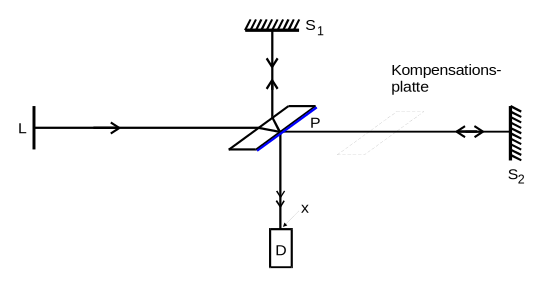
\includegraphics[width=0.8 \linewidth]{pictures/Michelson1.pdf}
    \caption{Der grundlegende Aufbau eines Michelson Interferometers. \cite{v401}}
    \label{fig:Michelson1}
\end{figure}

In \autoref{fig:Michelson1} ist schematisch der grundlegende Aufbau eines Michelson Interferometers dargestellt.
L ist dabei die Lichtquelle, also ein Laser. P ist eine semipermeable Platte, die dafür sorgt, dass das Licht
in zwei Strahlen aufgeteilt wird. Das bedeutet, dass ein Lichtstrahl zu Spiegel S$_1$ geht und der andere jeweils zu S$_2$.
An der Platte werden diese nun wieder zusammengeführt und laufen parallel zum Detektor D.\\
Da die beiden Strahlen kohärent sein müssen, muss der optische Wegunterschied kleiner als die Kohärenzlänge von L sein.
Um dies zu erreichen, wird der Abstand von den Spiegeln zu P fast identisch gewählt.
Würden die Längen exakt gleich gewählt werden, würde der Gangunterschied $\frac{\lambda}{2}$ betragen und
somit würde destruktive Interferenz vorliegen und die beiden Strahlen würden sich auslöschen.
Weiterhin wird eine Kompensationsplatte zwischen P und S$_2$ eingebaut, um den längeren Weg des Lichtstrahls nach S$_1$ zu kompensieren.
Der Lichtstrahl nach S$_1$ muss nämlich 3 Mal durch P durch, der andere jedoch nur einmal.\\
Wird nun ein Spiegel um die Länge $\increment d$ verschoben, ändert sich die Intensität am Schirm, beziehungsweise D.
Es gilt die Formel
\begin{equation} \label{eq:delta_d}
    \increment d = z \cdot \frac{\lambda}{2}.
\end{equation}
z beschreibt dabei die Anzahl der auftretenden Helligkeitsmaxima.


\subsection{Bestimmung des Brechungsindex n}

\begin{figure}
    \centering
    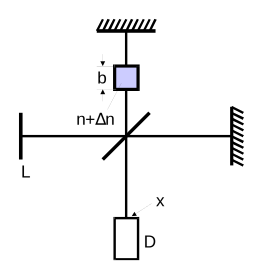
\includegraphics[width=0.4 \linewidth]{pictures/Michelson2.pdf}
    \caption{Der Aufbau eines Michelson Interferometers für die Messung eines Brechungsindizes. \cite{v401}}
    \label{fig:Michelson2}
\end{figure}

Mit der Apparatur lässt sich auch der Brechungsindex $n$ eines Mediums experimentell messen.
Dafür wird zunächst der Aufbau so wie in \autoref{fig:Michelson2} modifiziert. 
Der Lichtstrahl wird dann also durch das Medium der Länge $b$ mit dem Brechungsindex $n + \increment n$ geschickt.
Daraus ergibt sich dann der optische Wegunterschied von $ b \increment n$.
Dieser kann durch Evakuation des Gefäßes, oder auch durch Erhöhung des Druckes $p$, verändert werden.
Es gilt
\begin{equation}
    b \increment n = \frac{z \cdot \lambda}{2}.
\end{equation}
Für den Brechungsindex lässt sich durch die Dispersionstheorie 
\begin{equation}
    n = \sqrt{1 + f(\lambda) N}
\end{equation}
zeigen, wobei N die Zahl der von der Lichtwelle erzwungenen Schwingungen pro Volumeneinheit angeregten Dipolen beschreibt.
Im sichtbaren Bereich des Lichtes, kann die Formel mit
\begin{equation}
    n = 1 + \frac{f \cdot N}{2} - \dots
\end{equation}
genährt werden.
Unter der Annahme, dass die Gase sich wie ideale Gase verhalten, gilt
\begin{equation*}
    N (p, T) = \frac{p}{T}\frac{T_0}{p_0} N_L ,
\end{equation*}
wobei $T$ die Temperatur und $N_L$ die Loschmidtsche Zahl ist.
Durch einige Umformungen wird die Formel
\begin{equation} \label{eq:index}
    n\left(p_{0}, T_{0}\right)=1+\frac{z \lambda}{2 b} \frac{T}{T_{0}} \frac{p_{0}}{p-p^{\prime}}
\end{equation}
gewonnen.